%%%%%%%%%%%%%%%%%%%%%%%%%%%
%%% PART 2 - CHAPITRE 5 %%%
%%%%%%%%%%%%%%%%%%%%%%%%%%%

\chapter{Commençons par la mise en page}
\section{La structure d'un document}
Nous allons ici apprendre à hiérarchiser notre document selon son type.
\medskip

\begin{table}[h]
\begin{center}
\begin{tabular}{|c|c|}
\hline
\textbf{Élément de structure} & \textbf{Code \LaTeX} \\
\hline
Partie & \verb|\part{Titre de la partie}| \\
\hline 
Chapitre & \verb|\chapter{Titre du chapitre}| \\
\hline
Section & \verb|\section{Titre de la section}| \\
\hline
Sous-section & \verb|\subsection{Titre de la sous-section}| \\
\hline
Paragraphe & \verb|\paragraph{Titre du paragraphe}| \\
\hline
Sous-paragraphe & \verb|\subparagraph{Titre du sous-paragraphe}| \\
\hline
\end{tabular}
\caption{Les différents niveaux de hiérarchisation}
\end{center}
\end{table}
\medskip

A noter que fonction du type de document certains niveaux de hiérarchisation ne sont pas accessibles (Exemple: Le niveau \textit{Chapitre} n'est par accessible pour le type \texttt{book}).
\medskip

Exemple\footnote{Le texte de notre exemple est extrait de la page \textit{Wikipedia} de \LaTeX .}:
\begin{verbatim}
    \documentclass{report}

    \usepackage[french]{babel}
    \usepackage[utf8]{inputenc}
    \usepackage[T1]{fontenc}
    
    \begin{document}
    \part{Première partie}
    \chapter{Premier chapitre}
    \section{Première section}
    \subsection{Première sous-section}
    \LaTeX{} permet de rédiger des documents dont la mise 	en page 
    est réalisée automatiquement en se conformant 	du mieux 
    possible à des normes typographiques. Une 		fonctionnalité 
    distinctive de \LaTeX{} est son mode 		mathématique, qui permet 
    de composer des formules complexes... 
    \end{document}
\end{verbatim}
\bigskip

\section{Les annexes}
Avec le type de document \texttt{book} ou \texttt{report}, nous avons fréquemment besoin d'ajouter des annexes. \LaTeX{} offre la possibilité d'une numérotation différente de celle des chapitres. Entre le contenu du texte (et à fortiori des divers chapitres) et les annexes, on va insérer la commande \verb|\appendix|.
\medskip

Exemple:
\begin{verbatim}
    \chapter{Premier}
    \chapter{Deuxième}
    \chapter{Troisième}
    \appendix % Les annexes débutent ici
    \chapter{Une première annexe}
    \chapter{Une seconde annexe}
\end{verbatim}
\medskip

Avec le type \texttt{article} la commande \verb|\appendix| influera sur le titre des sections.
\medskip

\section{Modifier la numérotation}
Il est possible de créer des chapitres sans numéro, ni lettre, en insérant une étoiles dans la commande: \verb|chapter*{Titre du chapitre}|. Cela fonctionne avec tous les éléments de structure.
\medskip

Nous pouvons aussi modifier le comportement de la numérotation à l'aide des commandes suivantes:
\begin{description}
\item[\textbackslash frontmatter]: Positionnée juste après la commande \verb|\begin{document}|, elle permet de numéroter le préambule en chiffres romains.
\item[\textbackslash mainmatter]: Entre le préambule et le premier chapitre, elle permet de lancer la numérotation habituelle des pages (en chiffres arabes).
\item[\textbackslash backmatter]: Positionnée avant le chapitre épilogue, les index et la bibliographie, elle stoppe la numérotation des chapitres, mais pas celle des pages.
\end{description}
\medskip

\section{Page de garde}
Elle se compose de trois éléments:
\begin{description}
\item[Le titre du document]: \verb|\title{Titre du document}|
\item[Le nom de l'auteur]: \verb|\author{Nom de l'auteur}|
\item[Une date]: \verb|\date{La date voulue}|
\end{description}
\medskip

Ces trois éléments sont insérés avec avant la commande \verb|\begin{document}|, et la commande \verb|\maketitle| placée juste après \verb|\begin{document}| permet de composer la page de garde. Il est bien sûr possible de réaliser des pages de garde bien plus complexes.
\medskip

\section{Les alignements de texte}
Avec \LaTeX{} les paragraphes sont naturellement justifiés. Ainsi pour tout autre type d'alignements les environnements suivants sont disponibles:
\begin{description}
\item[L'environnement \texttt{flushright}]: alignement du texte à droite.
\item[L'environnement \texttt{center}]: pour centrer le texte.
\item[L'environnement \texttt{flushleft}]: alignement du texte à gauche.
\end{description}
\medskip

\section{Les sauts de lignes}
Sauter deux lignes permet de créer un paragraphe:
\begin{verbatim}
    \begin{document}
    Un premier paragraphe
    
    Un second paragraphe
    \end{document}
\end{verbatim}
\medskip

Pour aller à la ligne sans crée de nouveau paragraphe on utilise la commande \verb|\newline| ou bien \verb|\\|. Pour faire un saut de page, c'est la commande \verb|\newpage|.
\medskip

\section{La commande \texttt{\textbackslash documentclass\{\}}}
\begin{table}[h]
\begin{center}
\begin{tabular}{|p{3.25cm}|p{4cm}|p{3.25cm}|}
\hline
\textbf{Description} & \textbf{Valeurs applicables} & \textbf{Valeur par défaut} \\
\hline
Format du papier & \texttt{a4paper}, \texttt{a5paper}, \texttt{letterpaper}, \texttt{b5paper}... & \texttt{letterpaper} \\
\hline
Taille de la police principale & \texttt{10pt}, \texttt{11pt}, \texttt{12pt} & \texttt{10pt} \\
\hline
Alignement des équations & \texttt{fleqn} (à gauche) & Centrées par défaut \\
\hline
Colonnes & \texttt{onecolumn}, \texttt{twocolumn} & \texttt{onecolumn} \\
\hline
Première page des chapitres & \texttt{openany}, \texttt{openright} & \texttt{openright} \\
\hline
Recto verso & \texttt{oneside}, \texttt{twoside} & \texttt{article} et \texttt{report}: \texttt{oneside} \& \texttt{book}: \texttt{twoside} \\
\hline
\end{tabular}
\caption{Options applicables à la commande \texttt{\textbackslash documentclass\{\}}}
\end{center}
\end{table}
\medskip

Il est tout à fait possible d'insérer plusieurs options à la fois, il suffit pour cela de les séparer par des virgules.
\medskip

\section{Les marges}
Pour modifier les marges nous allons tout d'abord utiliser la commande \verb|\layout| du package \textit{layout}. Saisir le code suivant et le compiler afin d'obtenir le \textit{layout} du document.
\begin{verbatim}
    \documentclass[a4paper,10pt]{book}

    \usepackage[french]{babel}
    \usepackage[utf8]{inputenc}
    \usepackage[T1]{fontenc}

    % packages additionnels
    \usepackage{layout}

    \begin{document}

    \layout

    \end{document}
\end{verbatim}
\medskip

\begin{table}[h]
\begin{center}
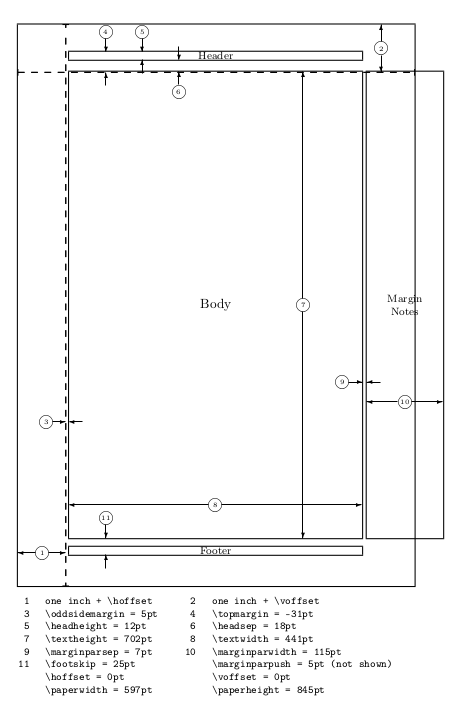
\includegraphics[scale=0.8]{IMG/layout.png}
\caption{Le \textit{layout}}
\end{center}
\end{table}
\medskip

Conjugué à un document saturé de texte nous pouvons visualiser le rendu avec les marges telles qu'elles sont définies. Nous pouvons alors modifier ces dernières à l'aide du package \textit{geometry}. Exemple de modification des marges à la fois en haut, en bas, à droite et à gauche, avec la ligne suivante placée dans la préambule du document:
\begin{verbatim}
    \usepackage[top=2.5cm, bottom=2.5cm, left=2.8cm, right=2.8cm]{geometry}
\end{verbatim}
\medskip

Il est toutefois possible d'intervenir encore plus finement en reprenant divers éléments du \textit{layout} qu'il est alors possible de modifier. Il suffit pour cela de placer dans le préambule une ligne du type:
\begin{verbatim}
    \setlength{nom_de_la_longueur}{longueur_dans_l'unité_voulue}
\end{verbatim}
\medskip

Un exemple:
\begin{verbatim}
    \setlength{\marginparwidth}{2cm}
\end{verbatim}
\medskip

\section{Les interlignes}
Les interlignes personnalisés s'obtiennent à l'aide du package \textit{setspace} et des commandes \verb|\onehalfspacing| et \verb|\doublespacing| qui permettent d'obtenir dans le document un interligne respectivement \textit{1,5} et \textit{2} fois plus grand que l'interligne habituel.
\medskip

Illustrons cela par le code suivant, à l'aide des environnement \texttt{onehalfspace} et \texttt{doublespace}:
\begin{verbatim}
    \documentclass[a4paper,11pt]{article}

    \usepackage[french]{babel}
    \usepackage[utf8]{inputenc}
    \usepackage[T1]{fontenc}

    \usepackage{setspace}

    \begin{document}
    \section{Interligne simple}
    \LaTeX{} est un langage et un système de composition de documents. 
    Il s'agit d'une collection de macro-commandes...
    
    \section{Interligne intermédiaire (\textit{1,5})}
    \begin{onehalfspace}
    \LaTeX{} est un langage et un système de composition de documents. Il 
    s'agit d'une collection de macro-commandes... 
    \end{onehalfspace}

    \section{Interligne double (\textit{2})}
    \begin{doublespace}
    \LaTeX{} est un langage et un système de composition de documents. Il 
    s'agit d'une collection de macro-commandes...
   \end{doublespace}
   \end{document}
\end{verbatim}
\medskip

\begin{table}[h]
\begin{center}
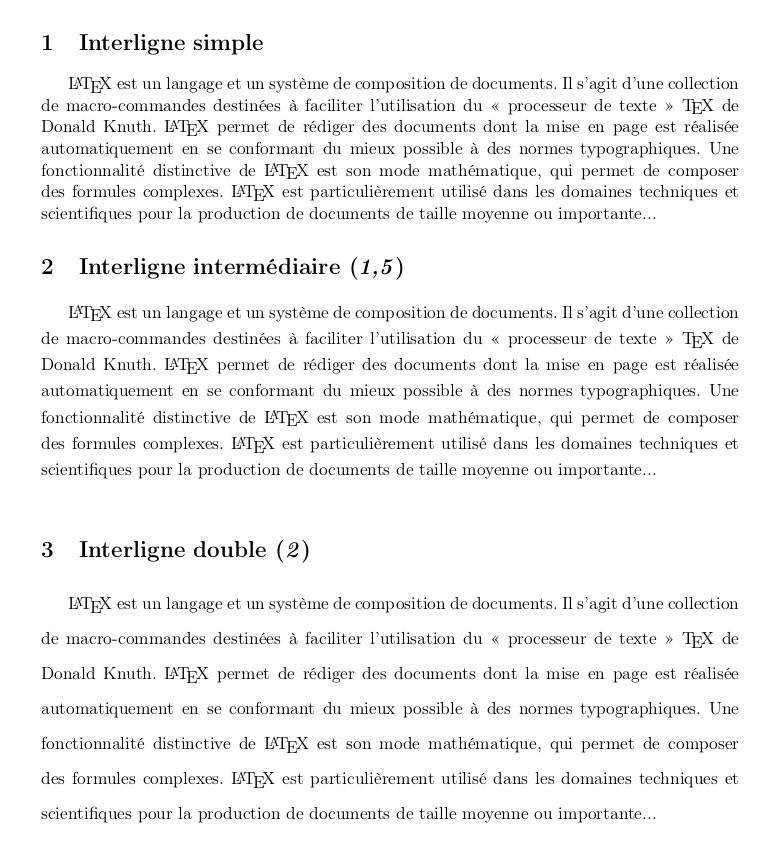
\includegraphics[scale=0.5]{IMG/interlignes.png}
\caption{Les interlignes}
\end{center}
\end{table}
\medskip

\section{Les listes}
Il existe les \textit{listes à puce}, les \textit{listes numérotées} et les \textit{les listes descriptives}. Chacune de ces listes s'insère dans un environnement spécifique. Plutôt que de partir sur de grandes explications, le principe étant aisé à comprendre, je vous propose de tester le code suivant:
\begin{verbatim}
    \documentclass[a4paper,11pt]{article}

    \usepackage[french]{babel}
    \usepackage[utf8]{inputenc}
    \usepackage[T1]{fontenc}

    \begin{document}
    \section{Les listes à puce}
    \begin{itemize}  % L'environnement des listes à puce
    \item Puce 1
    \item Puce 2
    \item Puce 3
    % Modifions les puces
    \item[@] Puce 4
    \item[5] Puce 5
    \item[*] Puce 6
    \item[\$] Puce 7
    \item[§] Puce 8
    \end{itemize}

    \section{Les listes numérotées}
    \begin{enumerate}  % L'environnement des listes numérotées
    \item Première
    \item Deuxième
    \item Troisième
    \end{enumerate}

    \section{Les listes descriptives}
    \begin{description}  % L'environnement des listes de description
    \item[Listes à puces]: avec l'environnement \textit{itemize}
    \item[Listes numérotées]: avec l'environnement \textit{enumerate}
    \item[Listes descriptives]: avec l'environnement \textit{description} 
    \end{description}
    \end{document}
\end{verbatim}
\medskip

\section{Les styles}
Pour peaufiner un peu plus nos mises en page nous allons voir maintenant les en-têtes et pieds de pages. De base, \LaTeX{} a été conçu avec trois modèles. Des packages proposent cependant des résultats plus aboutis, mais nous restons pour l'heure sur les modèles de base.
\medskip

Ces trois modèles sont donc:
\begin{description}
    \item[plain]: Ce style insère un numéro de page au milieu du pied de page.
    \item[headings]: Insère le nom du chapitre et le numéro de page en en-tête. Le pied de page demeure vide.
    \item[empty]: En-tête et pied de pages demeurent vides.
\end{description}
\medskip

Par défaut \LaTeX{} use du style \texttt{headings}. Pour modifier le style à une page en particulier, il suffit d'utiliser la commande \verb|\pagestyle{nom_du_style}| au début de la page.
\medskip

\section{Quelques règles}
Les commandes se terminant par des lettres doivent êtres suivies de la double accolade (\{\}) afin de pouvoir insérer une espace à leur suite (Exemple: \verb|\LaTeX{}|).
\medskip
